\cleardoublepage\chapter{State of the Art}\label{sec:sota}\minitoc\vspace{.5cm}\index{SotA}
This chapter provides a comprehensive and technical explanation of the aforementioned technologies mentioned earlier. 
The detail of DPDK and SR-IOV and their usage in current 5G system will be introduced in more detail.
Subsequently, the chapter presents the fundamental concept and design of eBPF and AF\_XDP, which is crucial for the implementation of the MTX library.

\section{DPDK: Data Plane Development Kit}
\ac{dpdkpage} is a library initially developed by Intel engineer Venky Venkatesan and currently maintained by the Linux Foundation. 
It provides a solution that contains a collection of libraries, poll drivers and configuration designed to accelerate packet processing workloads. 
By decoupling the NIC and CPU cores from the kernel, the library establishes a highly efficient and high-throughput data path, thus eliminates the overhead introduced by Linux kernel's network stack \cite{kourtis_enhancing_2015}. 
\ac{dpdkpage} has been widely utilized in various projects, including pfSense, Open vSwitch/OpenStack, Intel's DDP, OpenFlow, and 5G UPF implementations \cite{intel_ddp_ethernet_800}\cite{pongracz_removing_2013}\cite{zte_5g_core_upf_impl}\cite{nec_upf_whitepaper}. 
\\

From a technical standpoint, \ac{dpdkpage} is a complex kernel-bypassing library to process network packets that can deliver packets to application in user space with very low latency.
In addition, \ac{dpdkpage} offers a range of powerful features, including Crypto, DMA direct memory access, CUDA GPU utilization, and Machine Learning Device Driver \cite{dpdk_guide_page}. 
\ac{dpdkpage} is however, not a networking stack and has no Layer-3 forward, IPsec, firewall features \cite{old_dpdk_page}, thus forces developers to maintain their own code base for such purposes.
Therefore, using \ac{dpdkpage} in small open-source projects may necessitate more extensive maintenance and configuration compared to utilizing an in-kernel alternative like \ac{xdppage} socket, which will be utilized to construct our MTX library.
Unlike \ac{dpdkpage}, \ac{xdppage} socket has no monopoly on the \ac{NIC}, thus allows the kernel to manage and share the hardware resource to other applications.

\section{SR-IOV: Single Root I/O Virtualization}
\begin{figure}[H]
	\centering
	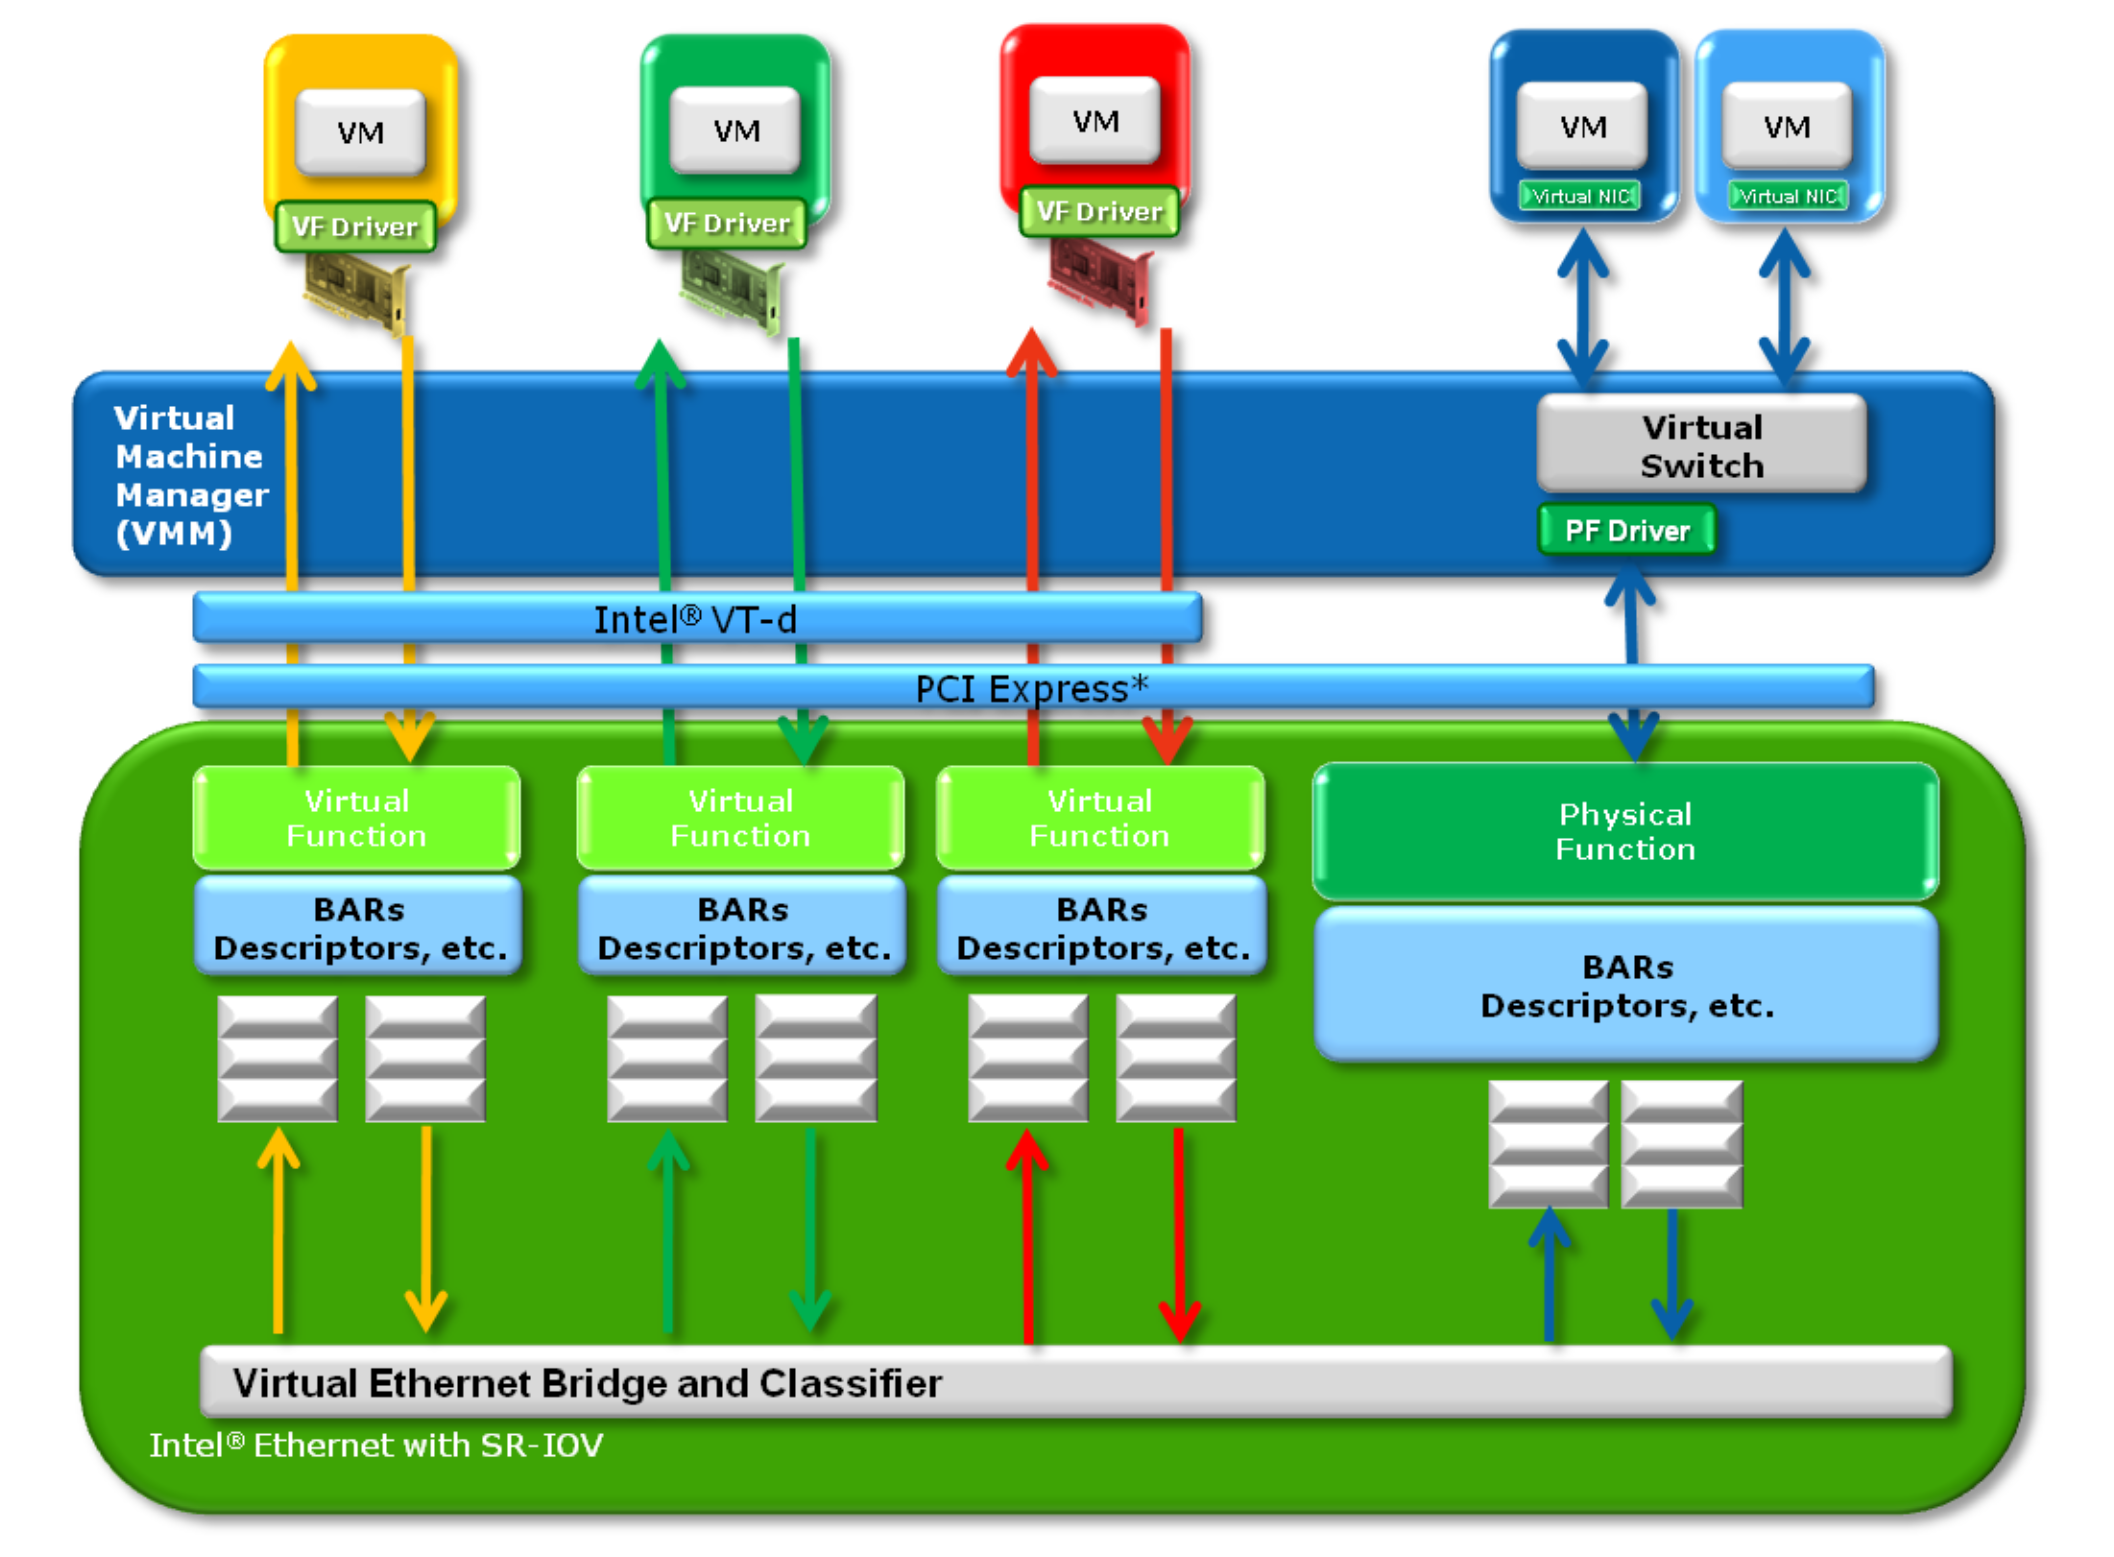
\includegraphics[width=1.0\textwidth]{resources/images/intel_sriov_Natively_and_Software_Shared.PNG}
	\caption{Natively (3 virtual machines on the left) and Software Shared \cite{intel_sriov}. The function type \textit{Virtual Function} (VF) can access a limited set of Base Address Register (BAR) descriptors (which holds the address of mapped memory of the device, or so called configuration space) and other parameters compared to the type \textit{Physical Function}. VF is designed to provide only the resources necessary for data movement.}
    \label{fig:sota:intel_sriov_Natively_and_Software_Shared}
\end{figure}

\ac{sriov} is a \ac{PCIe} specification that allows a physical \ac{PCIe} device to be partitioned into logical devices which appear as multiple physical devices in the guest \ac{OS} \cite{ibm_sriov}\cite{vmware_sriov}. 
By providing independent memory space, interrupts, and \ac{DMA} streams for each virtual machine, the natively shared devices achieve low latency and lower CPU utilization compared to virtual devices provided by traditional \ac{VMM}'s Virtual Switch or  I/O emulation layer (see \Cref{fig:related_work:intel_sriov_Natively_and_Software_Shared}) \cite{intel_sriov}.
As the \ac{sriov} specification is developed by \ac{PCISIGfootnote}, the consortium responsible for the \ac{PCIe} standard, there is no risk of vendor lock-in or significantly hidden cost.
A similar but less sophisticated method - namely \ac{PCIe} passthrough - to eliminates emulation overhead on I/O operation in hypervisor environment is completely disconnecting the \ac{PCIe} device from the host kernel and connecting it to the guest \ac{OS} instead, although this makes device sharing impossible.
It is also important to note that the \ac{sriov} specification is specifically designed for passing resources to and from a hypervisor environment, which is not conflict with our intended scenario.
The \ac{MTX} is designed as a general-purpose multipath tunnel that functions on \ac{NIC}s, making \ac{sriov} technology the underlying infrastructure layer for enabling \ac{MTX}'s \ac{xdppage} sockets to operate on the native shared devices.
This is similar to how \ac{ZTE} used \ac{sriov} in conjunction with \ac{dpdkpage} in their software stack \cite{zte_upf_full_whitepaper}.
\\

The Data plane relies on \ac{gptu} protocol with \ac{UDP} as the transport protocol to deliver high volume of data between \ac{UE} and \ac{DN} (see \Cref{fig:introduction:3gpp_5g_data_plane_protocol}), which require powerful processing power and high capable network link.
According to \ac{3GPP}, an non-exhausted list of \ac{UPF}'s responsibility is \textit{packet routing \& forwarding}, packet \textit{inspection}, \textit{buffering}, \textit{sending} and \textit{forwarding} \cite{3gpp_5g_system_architect_spec_release_18}.
In order to meet the \ac{SLA} and \ac{QoS} requirements, the \ac{UPF} needs to be deployed in various locations, such as the edge (edge and campus), regional sites, and central data centers. 
The size and form of each \ac{UPF} instance vary significantly depending on factors such as the number and size of downstream and upstream functions it manages and responds to \cite{zte_upf_full_whitepaper}.

\section{Current 5G deployment}
\begin{figure}[H]
    \centering
    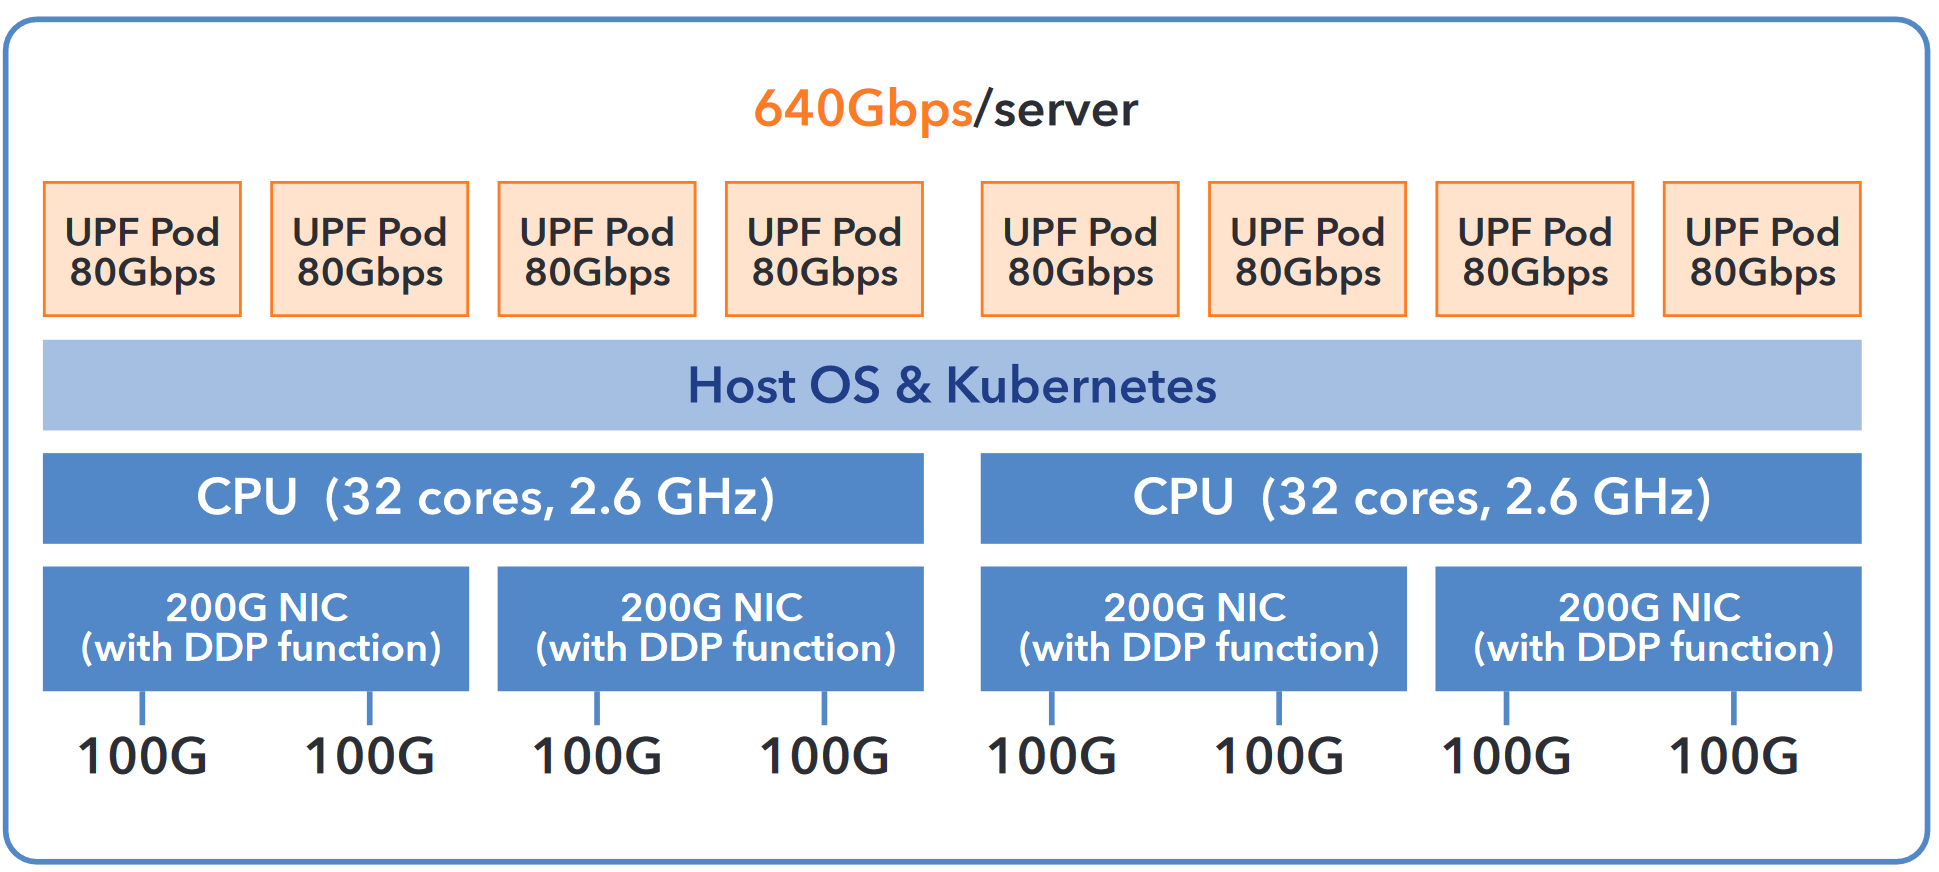
\includegraphics[width=0.6\textwidth]{resources/images/640_nec_upf_system.PNG}
    \caption{NEC's containerized UPF software (8 pods per server) on a platform configured with Linux and Kubernetes \cite{nec_upf_whitepaper}}
    \label{fig:sota:640_nec_upf_system}
\end{figure}
% \begin{figure}[H]
% 	\centering
% 	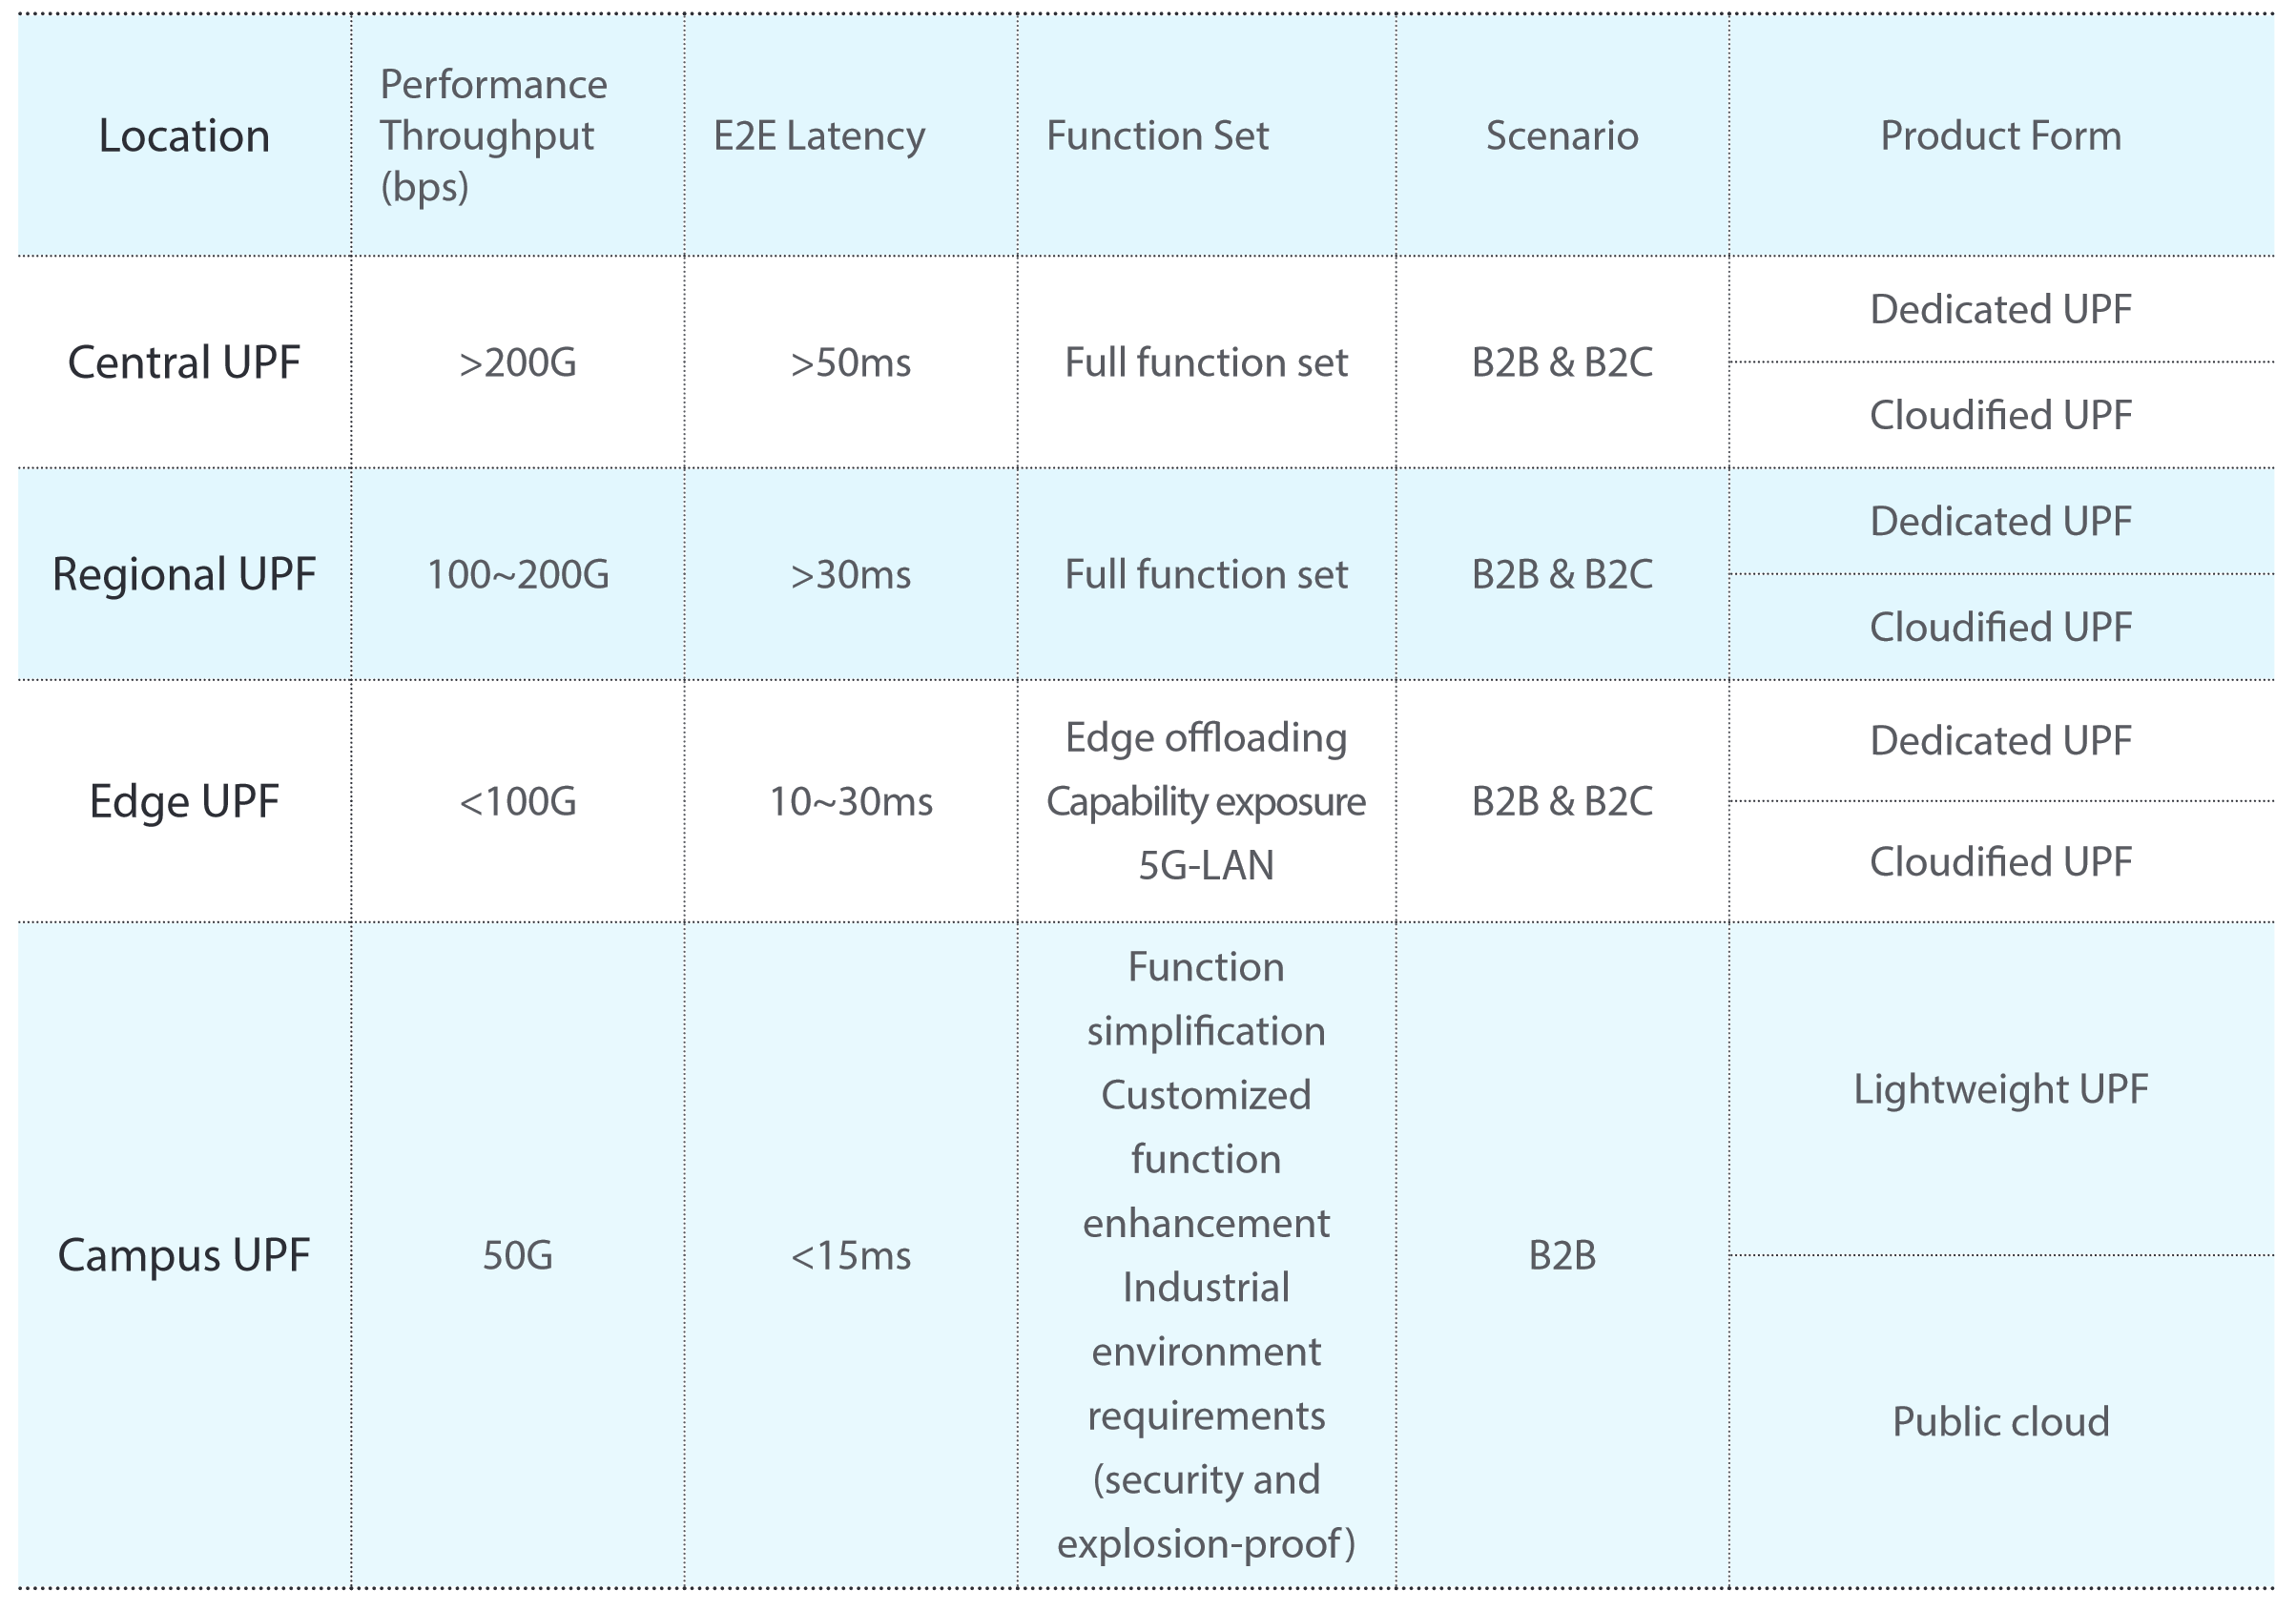
\includegraphics[width=1.0\textwidth]{resources/images/Deployment_Requirements_of_Full_Scenario_UPF.PNG}
% 	\caption{ZTE's White Paper: Deployment Requirements of Full-Scenario UPF \cite{zte_upf_full_whitepaper}}
%     \label{fig:sota:Deployment_Requirements_of_Full_Scenario_UPF}
% \end{figure}

It is common to see 5G services to be implemented and deployed in containers.
The underlying system often manage the containers using an orchestrator, i.e Kubernetes (\Cref{fig:sota:640_nec_upf_system}).

\section{XDP socket: AF\_XDP}
\subsection{Introduction to eBPF and Linux's kernel space}
The kernel functions as the central program of an operating system, overseeing its core operations. 
In a computer system, numerous processes execute concurrently, each fulfilling its assigned tasks. 
However, these processes possess limited access to its surrounding information and are inherently passive.
For instance, a process lacks the ability to initiate or terminate other processes, including itself. 
It operates in a isolated virtual memory and lacks direct communication channels with other processes or devices. 
Furthermore, it lacks awareness of its runtime availability, including when it can execute or must cease, as well as knowledge of its specific memory location, whether in RAM or swap.
Conversely, the kernel assumes the role of a housekeeper, managing the hardware resources of the computer and allocating them among all processes. It facilitates process execution, schedules runtime slots, and mediates communication and events between processes and hardware components.
In addition to these responsibilities, the kernel handles vital tasks such as memory management, providing a file system, establishing networking capabilities, and presenting the system's \ac{API} for programmatic access \cite{kerrisk_linux_2010}.
\\

Linux's virtual memory architecture divides the memory into two distinct spaces: kernel space and user space. This separation provides several advantages, such as enhancing system security and stability \cite{understanding_the_linux_kernel_bovet_cassetti}.
In Linux, tasks can operate in two distinct modes: kernel mode and user mode. When running in user mode, the CPU is restricted from accessing memory allocated for kernel space \cite{kerrisk_linux_2010}.
Invisible to end user, the system switches between kernel mode and user mode very often, usually when a system \ac{API} is involved or a resource needs to be accessed \cite{Robert_linux_kernel_dev}.
Although the CPU supports mode switching, there is a noticeable overhead associated with context switching and memory address translation. 
Running code exclusively in the kernel space has the potential to reduce this overhead and enjoy \textit{better} scheduling policies. 
However, such an approach carries inherent risks, including the possibility of system compromise due to memory leaks, crashes, or malicious exploits \cite{lwn_detect_kernel_mem_leak} \cite{emamdoost_detecting_2021}.
\\

\ac{BPF} technology provides an alternative means of executing code within the kernel space, offering a controlled environment for such operations. 
Initially introduced in 1992 for the \ac{BSD} OS, it was later ported to the Linux platform. 
Originally designed for network packet filtering, \ac{BPF} has since been expanded and utilized for purposes such as firewall management, tracing, and debugging \cite{McCanne_intro_bpf} \cite{lwn_intro_ebpf}. 
Prominent technology companies have leveraged \ac{BPF} for various applications, including: Facebook for firewall, filtering, and load balancing \cite{facebook_katran_ebpf_2018}; Netflix for network monitoring and analysis \cite{netflix_network_insight}; Cilium Project for security and observability purposes \cite{cilium_io_page} and Alibaba for their cloud infrastructure \cite{alibaba_cloud_ebpf}.
\\

\ac{ebpf} - the descendant of \ac{BPF} technology - consisted of a \ac{ebpf} program (also called \textit{kernel program}), the \ac{ebpf} virtual machine provided by the kernel, and the attach code path.
The \ac{ebpf} kernel program is written in a subset of the C programming language and compiled to \ac{ebpf} byte code.
The 64 bit \ac{RISC}-based \ac{ebpf} virtual machine along with a verifier check the code safety and isolate the execution of the \ac{ebpf} kernel program.
To get started, the kernel program is inserted to the desired code path in the kernel where it will be executed whenever the code path is traversed \cite{lwn_intro_ebpf}.

% \begin{figure}[H]
%     \centering
%     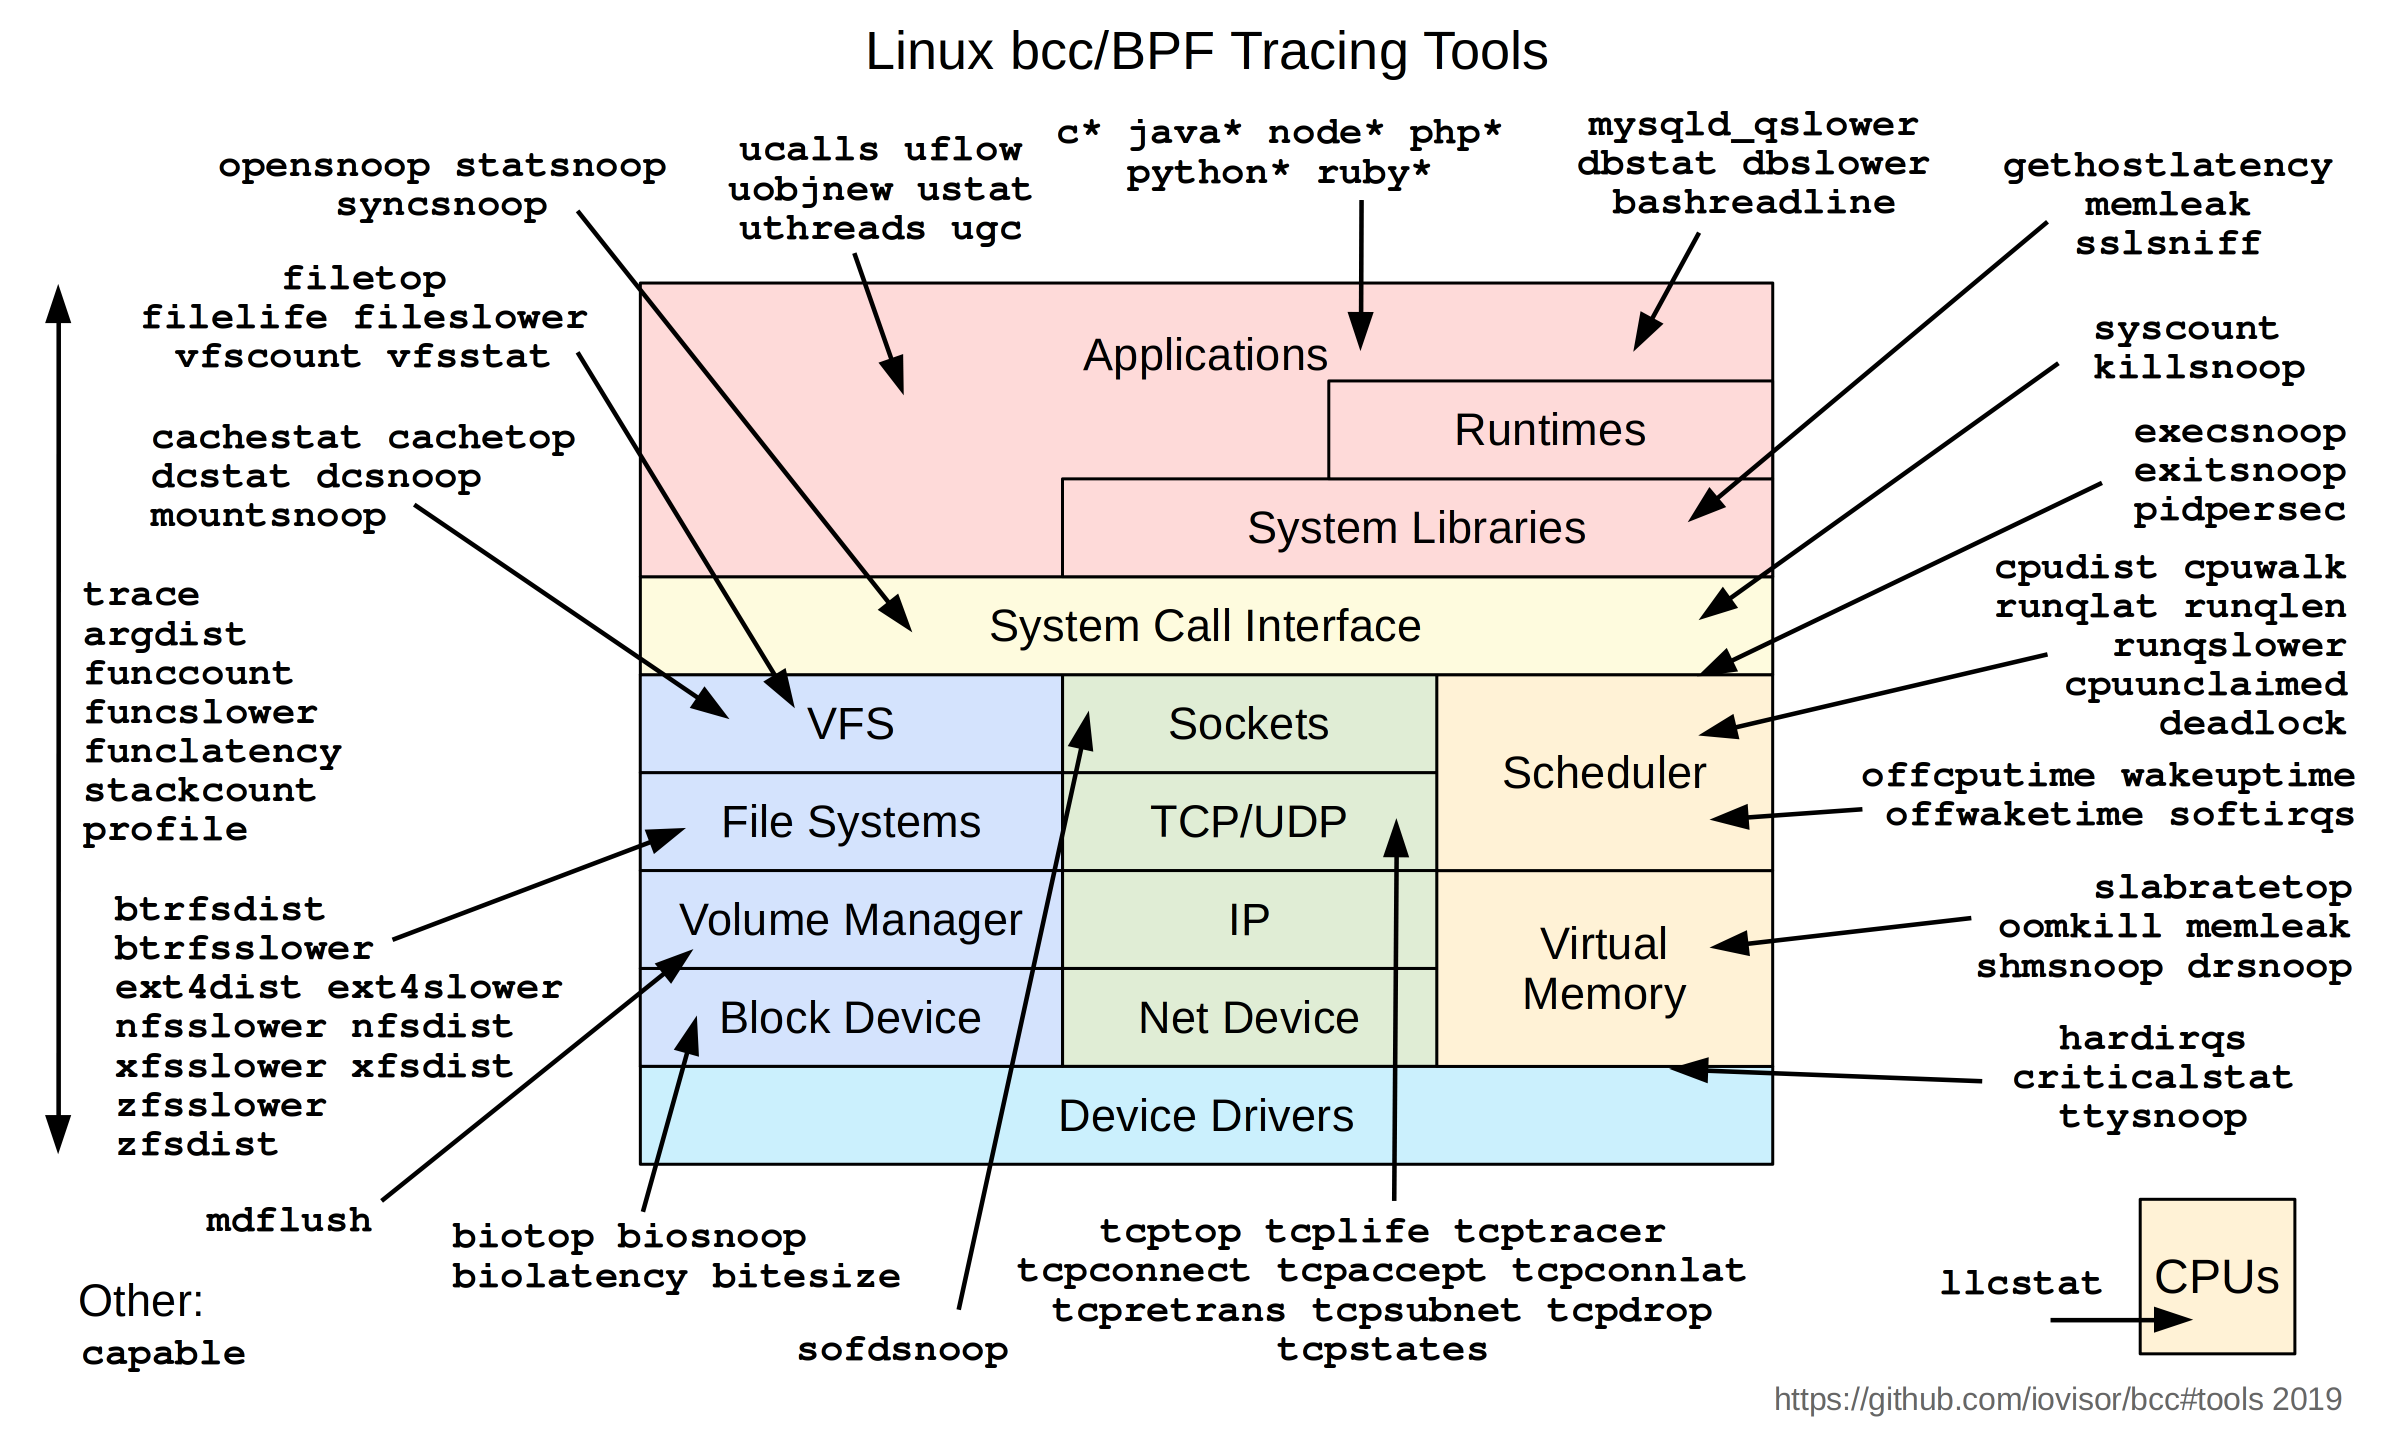
\includegraphics[width=1.0\textwidth]{resources/images/bcc_tracing_tools_2019.png}
%     \caption{A wide range of Linux eBPF-based tracing tools \cite{iovisor_page}.}\label{fig:sota:tracing_tools_linux}
% \end{figure}

\subsection{AF\_XDP socket}
\ac{xdppage} is a type of Linux socket that utilizes \ac{ebpf} to deliver incoming raw network packets arrived from a \ac{NIC} to user space with comparable performance to \ac{dpdkpage} \cite{karlsson_path_to_dpdk_speednodate}. 
The socket has demonstrated the capability to fully utilize a 100Gb line per core on modern CPUs, with impressive baseline packet drop rates of up to 24 million packets per second (Mpps) compared to 4.8Mpps with Linux network stack \cite{hoiland_jorgensen_express_2018} \cite{intel_dpdk_perf}.
This high throughput potential allows us to establish multi-hundreds Gb connections (tunnels) by leveraging a few readily available 40/100Gb NICs, presenting a valuable opportunity for enhanced network performance.

\begin{figure}[H]
	\centering
	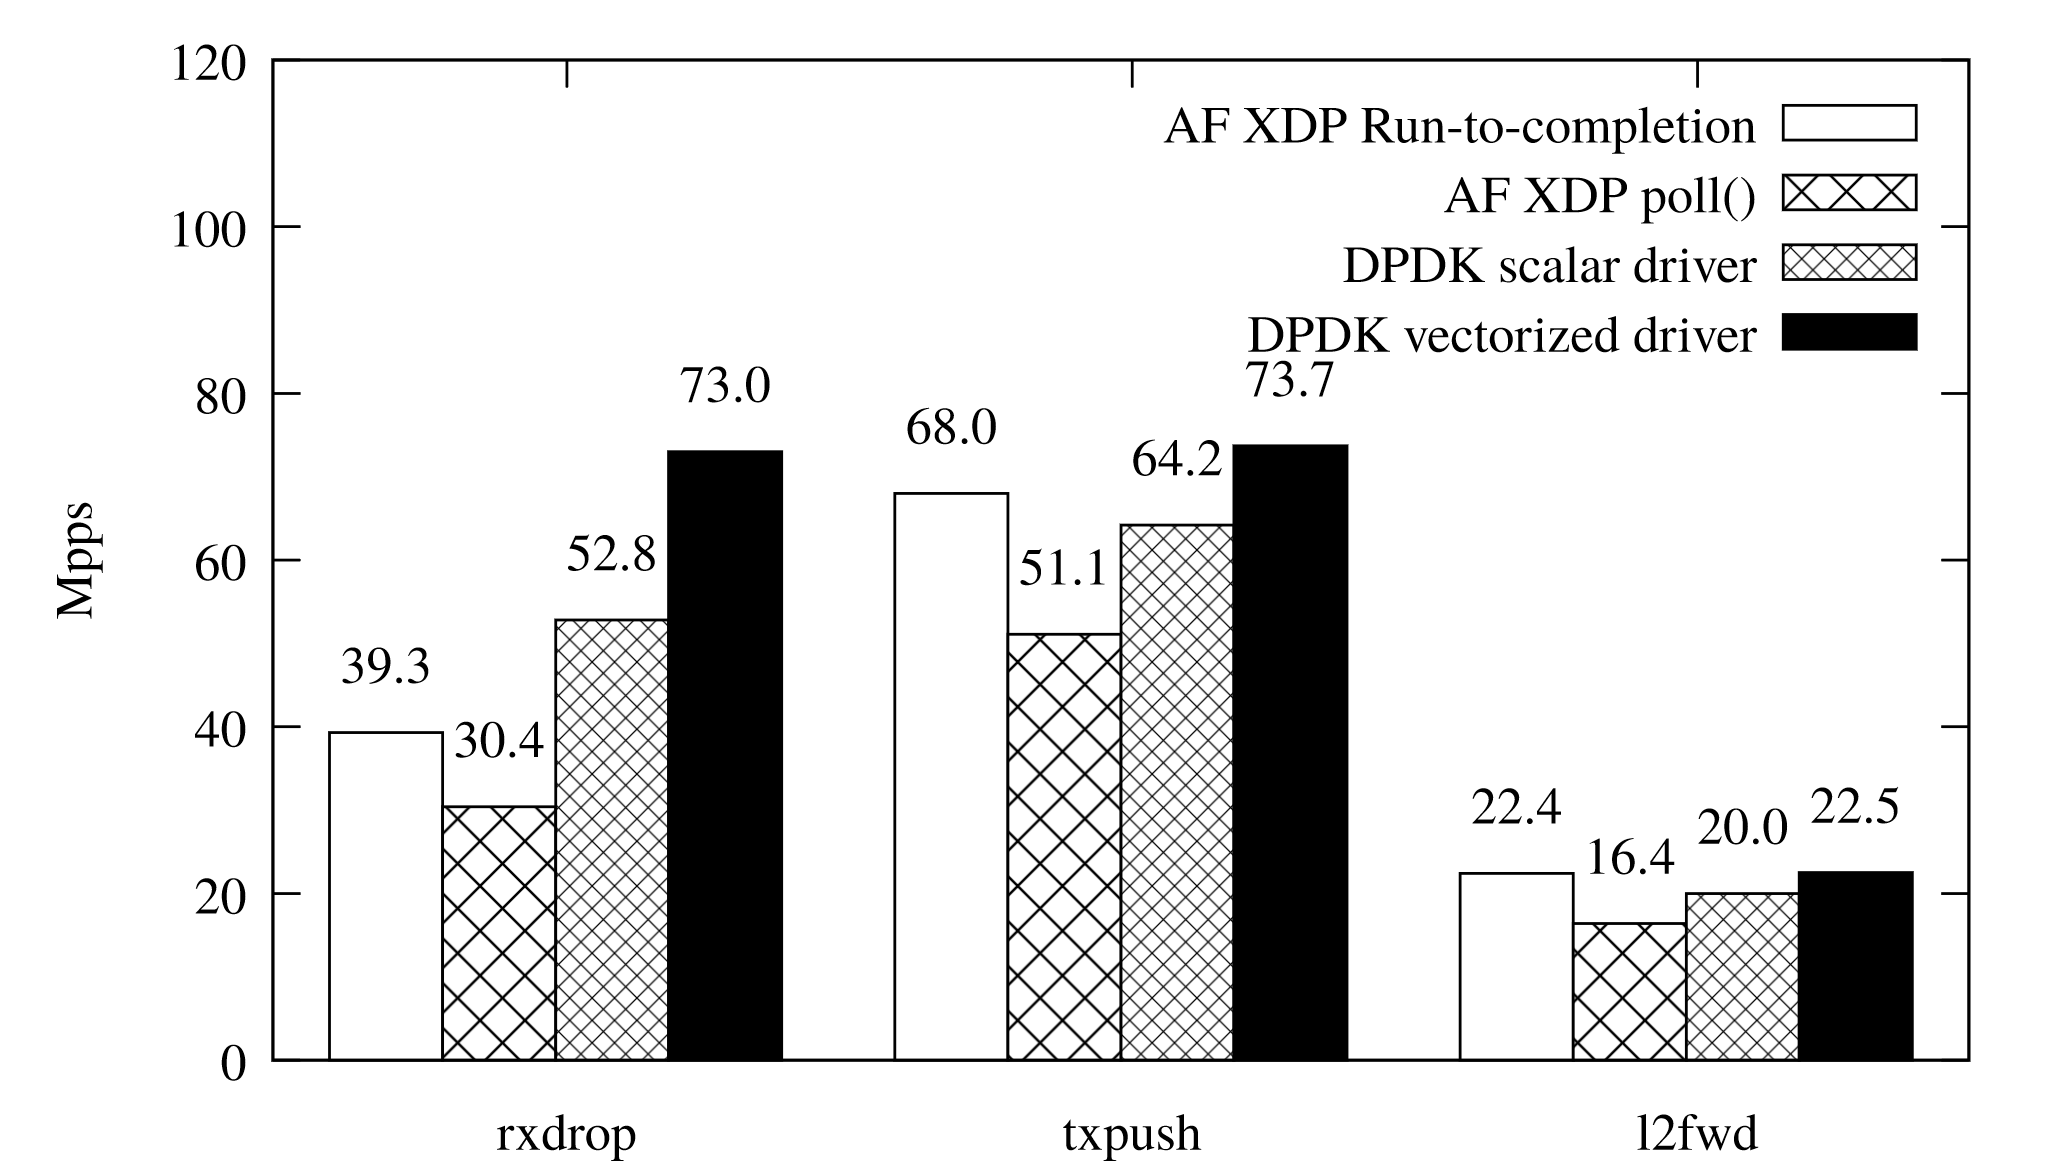
\includegraphics[width=0.8\textwidth]{af_xdp_vs_dpdk_3_micro_benchmarks.PNG}
	\caption{Comparing performance between \ac{xdppage} and \ac{dpdkpage} \cite{karlsson_path_to_dpdk_speednodate}. The authors tested  rxdrop (dropping all arriving packets), txpush (pushing packets out a NIC) and l2fwd (Level-2-forwarding, replacing MAC address of incoming packets and pushing them out) scenarios. DPDK continues to be the leading solution in terms of raw performance.}\label{fig:sota:af_xdp_vs_dpdk_3_micro_benchmarks}
\end{figure}

Being a native Linux's feature, \ac{xdppage} has several advantages over other 3rd party solutions:
\begin{itemize}
	\item Reducing dependency: minimizing the reliance on third-party libraries reduces the concern for potential vulnerabilities.Furthermore, this approach guarantees the longevity of the product, as the socket is maintained by the dedicated team of kernel developers, indicating that the project is unlikely to be discontinued in the near future. 
	\item License: no special license required. However, the eBPF kernel program must be licensed under GNU \ac{GPL} since anything uses eBPF in kernel space is considered a derivative work \cite{gpl_email_discussion} \cite{linux_license_rule} \cite{lwn_clarify_bpf_license}.
	\item Security and Update: the open-source and collaborative nature of Linux ensures that its code base is diligently maintained by dedicated maintainers and an active community of contributors, including researcher from universities and institutes, employee from industrial vendors and individual hobbyist.
\end{itemize}

% \begin{figure}[H]
% 	\centering
% 	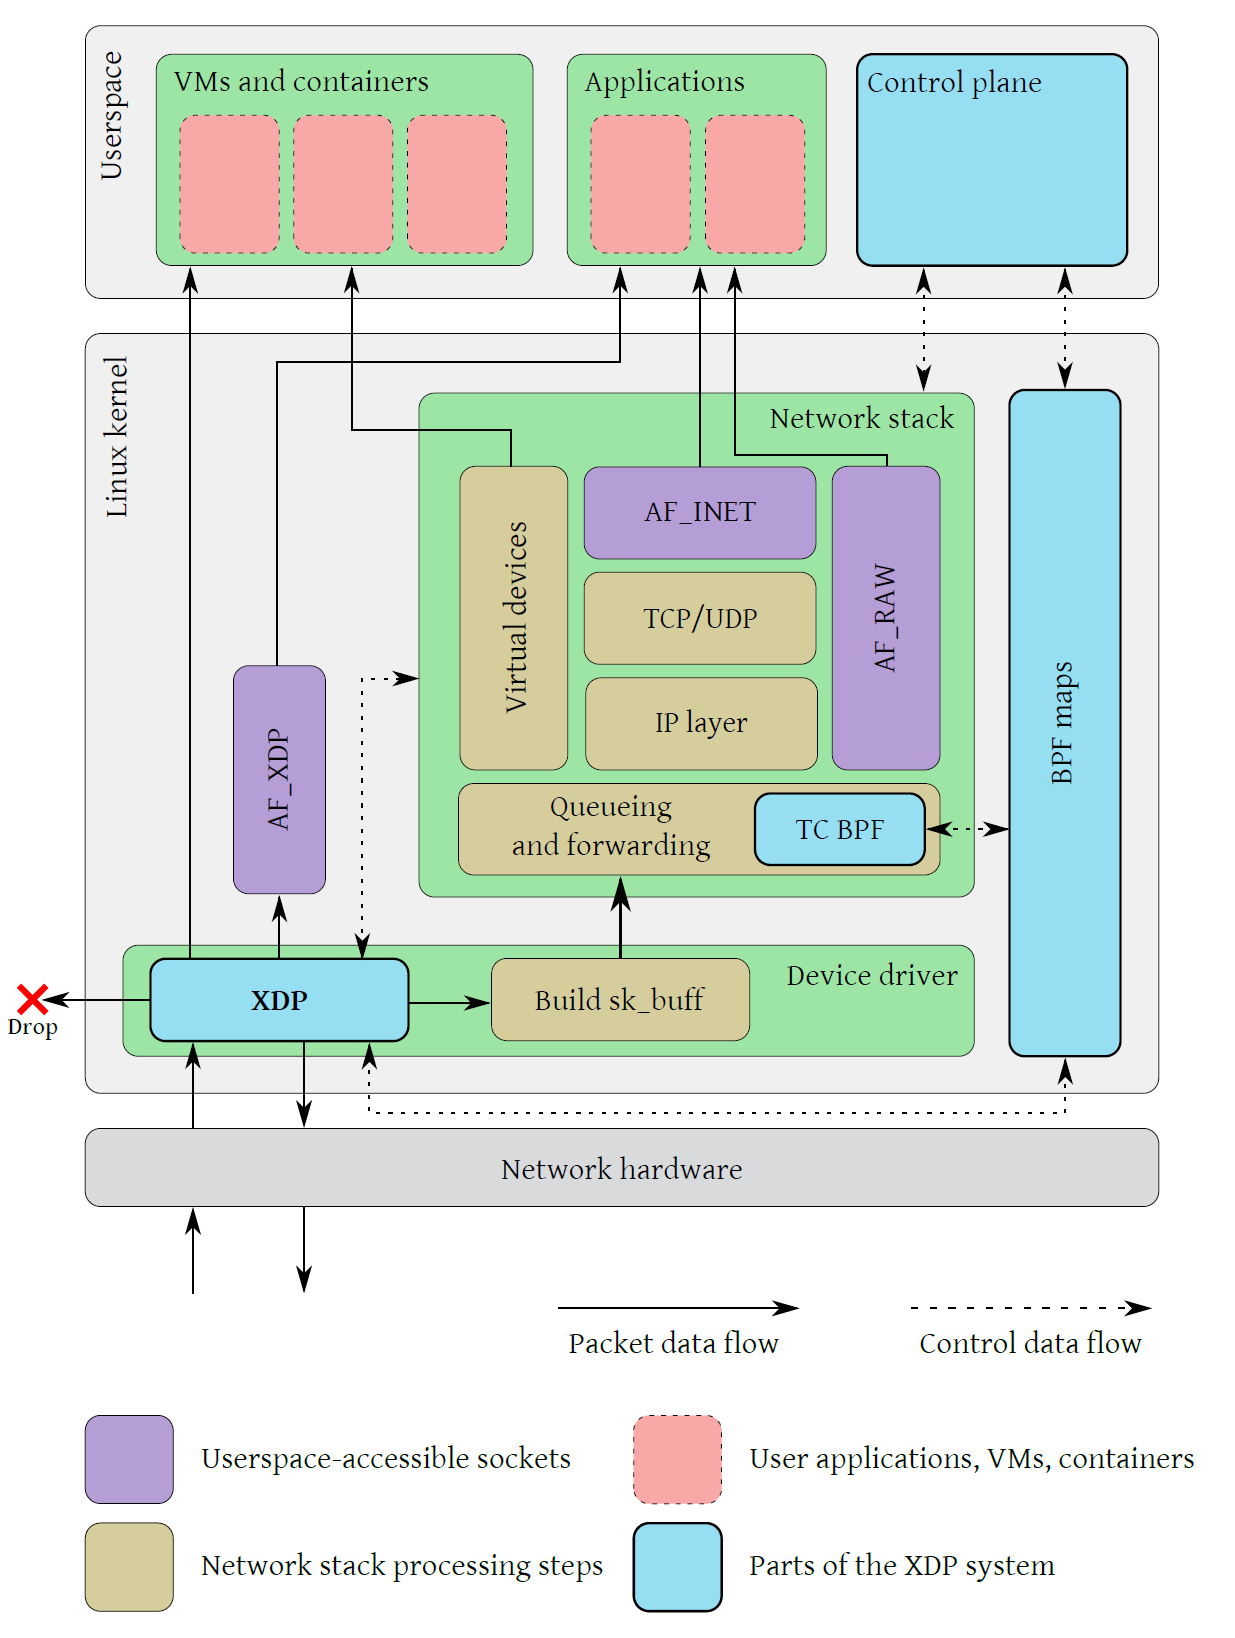
\includegraphics[width=1.0\textwidth]{XDP_integration_with_the_Linux_network_stack.PNG}
% 	\caption{XDP’s integration with the Linux network stack \cite{hoiland_jorgensen_express_2018}. The XDP program is activated whenever a packet enter the driver's buffer, where it will be examined. The XDP program makes the decision if the packet should follow its normal path in the network stack, or be discarded/forwarded/delivered to XDP user space program.}\label{fig:sota:xdp_architecture}
% \end{figure}

